\documentclass[conference]{../lib/IEEEtran}
\IEEEoverridecommandlockouts
% The preceding line is only needed to identify funding in the first footnote. If that is unneeded, please comment it out.
\usepackage{cite}
\usepackage{amsmath,amssymb,amsfonts}
\usepackage{algorithmic}
\usepackage{graphicx}
\usepackage{textcomp}
\usepackage{xcolor}
\def\BibTeX{{\rm B\kern-.05em{\sc i\kern-.025em b}\kern-.08em
    T\kern-.1667em\lower.7ex\hbox{E}\kern-.125emX}}

\usepackage{minted}

\usepackage{siunitx}
\DeclareSIUnit\sample{samples}

\usepackage{nonfloat}
\renewenvironment*{figure}[1][]
    {
        \minipage{\linewidth}
    }
    {
        \endminipage
        \\*[\intextsep]
    }
\renewenvironment*{table}[1][]
    {
        \minipage{\linewidth}
    }
    {
        \endminipage
        \\*[\intextsep]
    }
%--------------------------------------------------

\usepackage{mathtools}%
\DeclarePairedDelimiter\abs\lvert\rvert%
\DeclarePairedDelimiter\brao()%
\DeclarePairedDelimiter\brac[]%
\DeclarePairedDelimiter\braco[)%
\DeclarePairedDelimiter\braoc(]%
\DeclarePairedDelimiter\Brac\{\}%
\DeclarePairedDelimiter\angl<>%
\DeclarePairedDelimiter\floor\lfloor\rfloor%
\DeclarePairedDelimiter\piece\{.%

\newcommand*\hfrac[2]{#1/#2}
\newcommand*\tbrao[1]{(#1)}

\begin{document}

\title{ECE 4522 MATLAB Assignment 2}

\author{\IEEEauthorblockN{Leomar Dur\'an}
\IEEEauthorblockA{\textit{College of Engineering} \\
\textit{Temple University}\\
Philadelphia, PA \\
leomar.duran@temple.edu}
}

\maketitle

\begin{abstract}
This assignment introduces various types of systems and provides hands on experience with the impulse response. It cements the concept of convolution using MATLAB including effects on a sound sample, and expands it with the concept of a restoring system to undo convolution. We will find the error plot and worst-case error to compare out actual result with the expected input and prove that a restoring system is possible.
\end{abstract}

\begin{IEEEkeywords}
convolution, finite-duration impulse response, FIR, discrete-time system, echo system, restoration system, digital signal processing, cascading systems
\end{IEEEkeywords}

\section{Objectives}

The objectives of this report are to prove the concept of a restoring system and to provide a concrete example of an echo system on a sound sample.

After this lab, students will be able to identify various types of systems including echo systems, restoring systems, and cascading systems.

\section{Methods}

\mintinline{bash}{./Ece4522/MatlabAssignment2/A.m} is a template included in the specification demonstrating a simple convolution of a sinusoidal wave running through a running average system and plots the input and output.

\mintinline{bash}{./Ece4522/MatlabAssignment2/B1.m} has multiple parts. Part B.1, performs a similar convolution on a different wave. Part B.2 then performs a Restoration System which attempts to recover the original system. Part B.3 finds what the error (difference) in the worst-case was when the restoration was attempted. Finally, Part B.4 reads in a sound sample, applies a similar convolution to part B.1, and saves the result.

\mintinline{bash}{./Ece4522/MatlabAssignment2/C.m} applies two systems to be cascaded to an impulse signal, which will later be compared to the same cascade found mathematically.

\section{Results}

\subsection{Part B.1 FIR System}

\begin{figure}
    \centering
    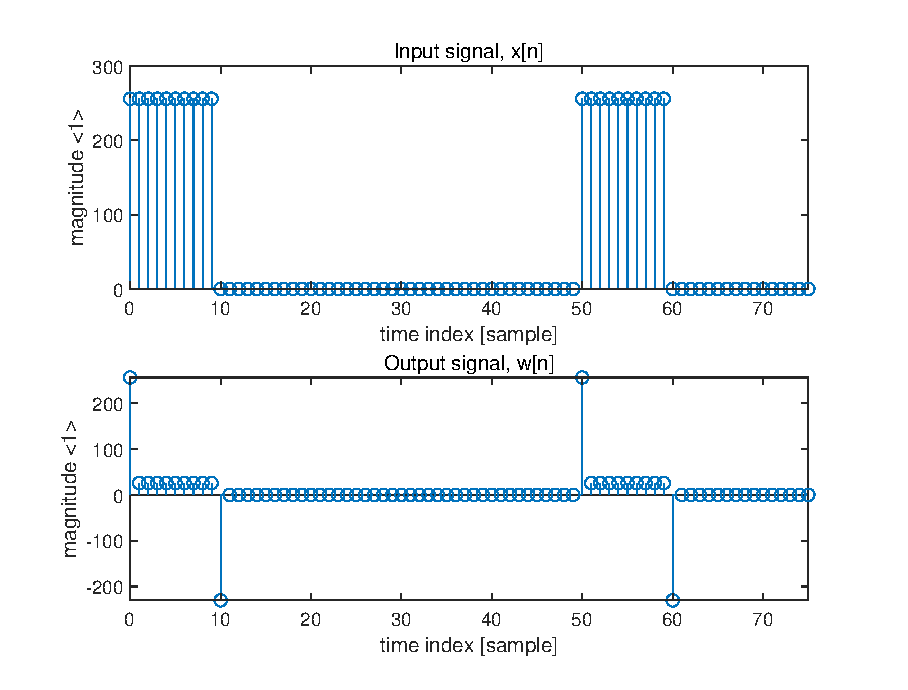
\includegraphics[width=\linewidth]{ece4522ma2fig1.eps}
    \figcaption{Input signal \(x\brao{n}\) and output signal \(w\brac{n}\) of an FIR system.}
    \label{fig:B.1-fig1}
\end{figure}

\subsection{Part B.2 Restoration System (b)}

\begin{figure}
    \centering
    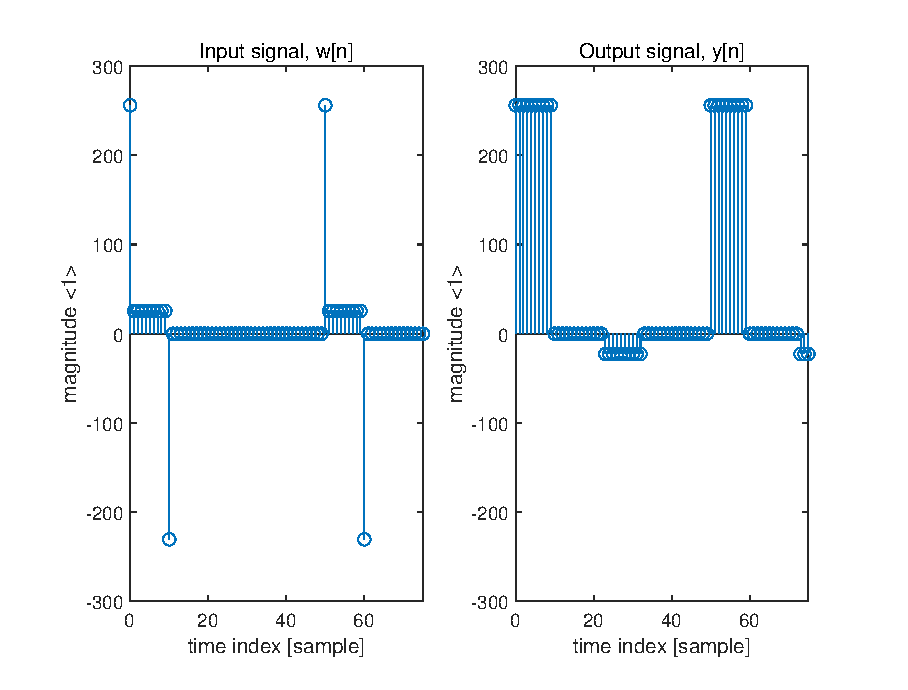
\includegraphics[width=\linewidth]{ece4522ma2fig2.eps}
    \figcaption{Input signal \(w\brao{n}\) and output signal \(y\brac{n}\) of a restoration system. This system aims to restore the signal \(x\brao{n}\).}
    \label{fig:B.2b-fig2}
\end{figure}

\subsection{Part B.2 Restoration System (c)}

\begin{figure}
    \centering
    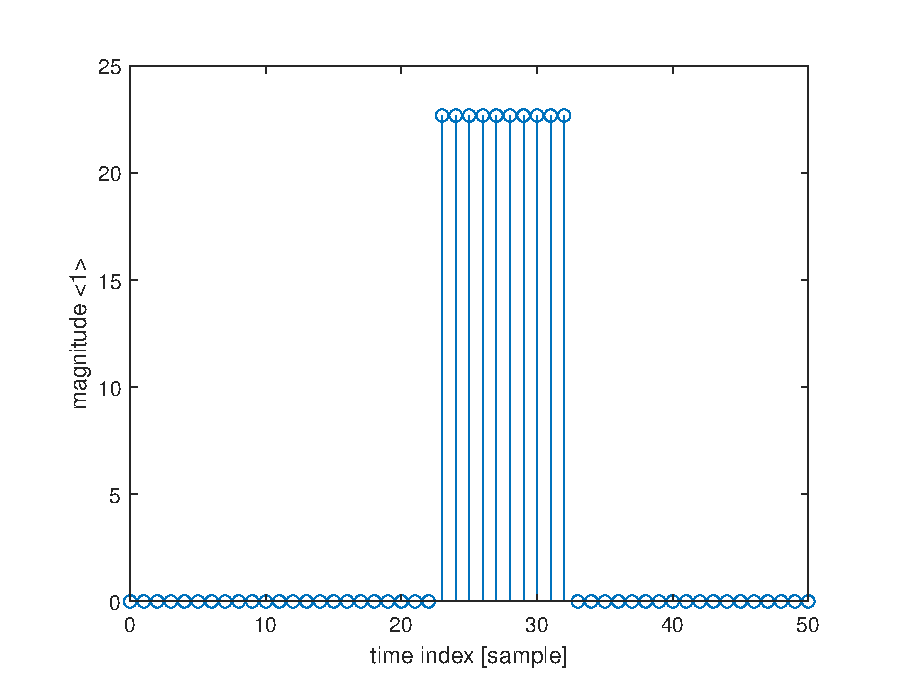
\includegraphics[width=\linewidth]{ece4522ma2fig3.eps}
    \figcaption{Error (difference) between \(y\brao{n}\) found in part B.2(b) and the original \(x\brao{n}\).}
    \label{fig:B.2c-fig3}
\end{figure}

\section{Insights}

\subsection{Part B.1 FIR System}

The input in Fig. \ref{fig:B.1-fig1} represents \(256\) times the remainder of \(n \in \mathbb{Z}[0..100]\) divided by \(50\). Whereas, the output is equivalent to the input at the current sample, subtracted by the input at the immediately previous sample attenuated to 0.9 times its amplitude.

Since the impulse response \( h\brac{n} := \brac{\begin{matrix} 1 & -0.9 \end{matrix}} \approx \brac{\begin{matrix} 1 & -0.9 & 0 & 0 & \cdots & 0 \end{matrix}}\), we find that
\[
    \begin{aligned}
        &y\brac{n}
    \\*
        {}:={}& \sum_{k = 0}^{M} h\brac{k}x\brac{n - k}
    \\*
        {}\hphantom:={}& 1x\brac{n\!-\!0} - 0.9 x\brac{n\!-\!1} + 0x\brao{n\!-\!2} + \cdots + 0x\brac{n\!-\!M}
    \\*
        {}\hphantom:={}& x[n] - 0.9 x[n - 1]
     \end{aligned}
\]
is the effect of the system impulse response on the input signal.

To find the length of this output signal, let's define \(\nu\brao{\vec{v}}\) as the length of the vector for any row vector \(\vec{v}\). Then \(\nu\brao{w\brac\cdot} = \nu\brao{x\brac\cdot} + \nu\brao{h\brac\cdot} - 1\). In this case, \(\nu\brao{w\brac\cdot} = \nu\brac{0..100} + \nu\brac{\begin{matrix} 1 & -0.9 \end{matrix}} - 1 = 101 + 2 - 1 = 102\).

\subsection{B.3 Worst-Case Error}

The error plot in Fig. \ref{fig:B.2c-fig3} shows the absolute difference between the original (and expected) signal \(x\brac{n}\) and the signal \(y\brac{n}\) that was received from the restoration system. It shows that when \(n \in \braco{0, 23} \cup \braoc{32, 50}\), the error is \(0\), but in \(22.6891\) when \(n \in \brac{23, 32}\). The worst-case error shows the maximum absolute error, which is in fact \(22.6891\). Compared to the amplitude, this is a rate of \(\frac{22.6891}{256} \approx 0.0886\), which is still very significant.

If the worst-case error had been of a much lower magnitude, at about \(\num{7.3e-15}\), such as the value at \(y\brac{22}\) then the difference with \(x\brac{n}\) would not be noticeable at all in its plot.

\subsection{Part B.4 An Echo System}

\(y_1\brac{n} = x_1\brac{n} + rx_1\brac{n - P}\) represents an echo system because it adds onto \(x_1\brac{n}\), a repetition delayed by \(P\) samples at a rate of \(r\) the original's strength as defined by an echo system.

To have a \(\SI{90}\percent\) strength echo delayed by \(0.2\) seconds, \(r := \SI{90}\percent = 0.9\). Now 
\[
	x_a\brao{t} = x_a\brao{nT} = x_1\brac{n}.
\]
Then \(t - \SI{0.2}\second = \brao{n - P}T = nT - PT\). So \(\SI{0.2}\second = PT = \hfrac{P}{\SI{8000}\hertz}\). Thus \(P := \brao{\SI{0.2}\second}\brao{\SI{8000}\hertz} = \SI{1600}\sample\).

So a \(r := 0.9\) and \(P := \SI{1600}\sample\) will satisfy the requirements for this system.

Now, the impulse response of the echo system
\[
	h\brac{n} = \delta\brac{n} + r\delta\brac{n - P} := \piece*{
		\begin{array}{@{}*2l@{}}
			1 & \text{if \(n = 0\)};\\*
			0.9 & \text{if \(n = 1600\)};\\*
			0 & \text{otherwise}.\\*
		\end{array}
	}
\]
and the length \(\nu\brao{h\brac\cdot} = P + 1 = 1600 + 1 = 1601\).

\subsection{Part C. Cascading Two Systems}

Since FIR System-1 impulse response \(h_1\brac{n} := \brac{\begin{matrix}1 & -q\end{matrix}} \approx \brac{\begin{matrix}1 & -q & 0 & 0 & \cdots & 0\end{matrix}}\), then the overall impulse response
\[
    \begin{aligned}
            &h\brac{n}
    \\*
        :={}& \sum_{\ell=0}^{M} r^\ell h_1\brac{n - \ell}
    \\*
        \hphantom:={}& \sum_{\ell=0}^{M} h_1\brac\ell r^{\brao{n - \ell}} \qquad \text{by commutativity}.
    \\*
        \hphantom:={}& 1 r^{\brao{n - 0}} - qr^{\brao{n - 1}}
    \\*
        \hphantom:={}& r^n - qr^{\brao{n - 1}}.
    \\*
    \end{aligned}
\]

Well \(h\brac0 = 0.9^0 = 1\) and \(h\brac{m} = 0.9^m - 0.9\brao{0.9^{\brao{m - 1}}} = 0.9^m - 0.9^m = 0\) for all \(m \not= 0\).

Thus the overall impulse response \begin{eqnarray}h\brac{n} = \brac{\begin{matrix} 1 \end{matrix}},\label{eqn:hn-1}\end{eqnarray} the impulse signal.

Now for an impulse signal to give \(y\brac{n} = \sum_{k=0}^M h\brac{k}x\brac{n-k} = x\brac{n}\), note that it's the case that
\[
x\brac{n} = 1x\brac{n-0} + 0x\brac{n-1} + 0x\brac{n-2} + \cdots + 0x\brac{n-M}.
\]
So \[1x\brac{n-0} + 0x\brac{n-1} \cdots + 0x\brac{n-M} = \sum_{k=0}^M h\brac{k}x\brac{n-k}. \]
So \(h\brac{n} = \brac{\begin{matrix}1\end{matrix}} = \brao{h_1\ast h_2}\brac{n} \Longleftrightarrow: P\brao{h_1, h_2}\).

As found in the \textsc{Matlab} script mathematically resulting in equation \tbrao{\ref{eqn:hn-1}}, it is the case that the FIR System-1 represented by \(h_1\brac\cdot\) and the FIR System-2 represented by \(h_2\brac\cdot\) do meet the condition expressed by \(P\brao{h_1,h_2}\).

\section{Conclusion}

We have proven that it is mathematically possible for two systems \(h_1\brac\cdot, h_2\brac\cdot\) to create cascade with the latter forming a restorative system as long as they satisfy \(P\brao{h_1, h_2} :\Leftrightarrow \brao{h_1\ast h_2}\brac{n} = \brac{\begin{matrix}1\end{matrix}}\).

We have also identified moving average and echo impulse responses, and demonstrated cascading systems.

\end{document}
